\documentclass{beamer}

\usetheme{metropolis}

\usepackage{graphicx}
\usepackage{booktabs}
\usepackage{tikz}
\usepackage{xcolor}

\definecolor{mainblue}{RGB}{0,102,204}

\setbeamercolor{alerted text}{fg=mainblue}
\setbeamercolor{block title}{bg=mainblue!20,fg=black}
\setbeamercolor{block body}{bg=mainblue!5,fg=black}

\title{Mini Project Presentation}
\subtitle{Hostel Issue Management System (HostelPulse)}
\author{
Abhinav Singh (2400520100004) \\
Ansh Sharma (2400520100016) \\
Bhavya Nigam (2400520100028) \\
Devraj Gupta (2400520100034) \\
Himanshu (2400520100040)
}
\date{\today}

\begin{document}

%--------------------------------
\begin{frame}
\titlepage
\end{frame}

%--------------------------------
\begin{frame}{Project Overview}

\begin{block}{What is HostelPulse?}
HostelPulse is a web-based platform designed to simplify reporting
and managing hostel-related issues.
\end{block}

\begin{columns}

\column{0.48\textwidth}

\begin{alertblock}{Problem}
\begin{itemize}
\item Complaints reported manually
\item No centralized tracking
\item Delayed issue resolution
\end{itemize}
\end{alertblock}

\column{0.48\textwidth}

\begin{block}{Solution}
\begin{itemize}
\item Online complaint submission
\item Admin management dashboard
\item Transparent issue tracking
\end{itemize}
\end{block}

\end{columns}

\end{frame}

%--------------------------------
\begin{frame}{Technology Stack}

\begin{columns}

\column{0.5\textwidth}

\begin{block}{Frontend}
\begin{itemize}
\item React
\item Tailwind CSS
\end{itemize}
\end{block}

\begin{block}{Backend}
\begin{itemize}
\item Node.js
\item Express.js
\end{itemize}
\end{block}

\column{0.5\textwidth}

\begin{block}{Database}
\begin{itemize}
\item MongoDB
\end{itemize}
\end{block}

\begin{block}{Security \& Deployment}
\begin{itemize}
\item JWT Authentication
\item GitHub
\item Vercel (Frontend)
\item Render (Backend)
\end{itemize}
\end{block}

\end{columns}

\end{frame}

%--------------------------------
\begin{frame}{System Architecture}

\begin{center}
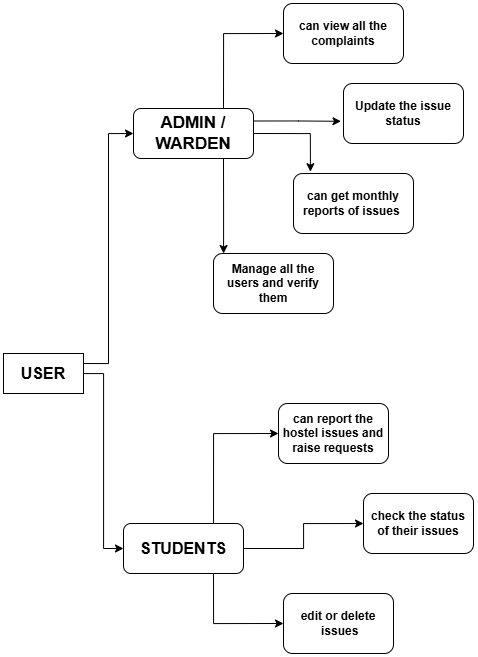
\includegraphics[height=0.85\textheight]{architecture1.drawio.png}
\end{center}

\end{frame}

%--------------------------------
\begin{frame}{System Flow}

\begin{center}

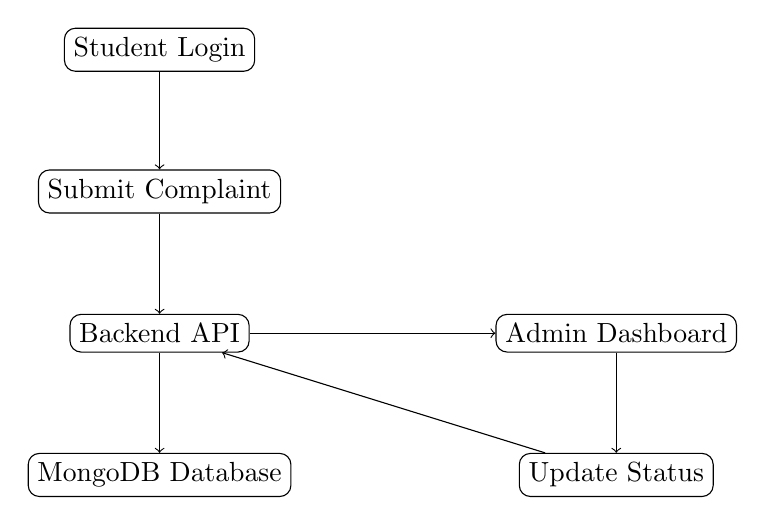
\begin{tikzpicture}[node distance=1.8cm,
every node/.style={draw, rounded corners, align=center}]

\node (login) {Student Login};
\node (submit) [below of=login] {Submit Complaint};
\node (backend) [below of=submit] {Backend API};
\node (db) [below of=backend] {MongoDB Database};

\node (admin) [right of=backend, xshift=4cm] {Admin Dashboard};
\node (update) [below of=admin] {Update Status};

\draw[->] (login) -- (submit);
\draw[->] (submit) -- (backend);
\draw[->] (backend) -- (db);

\draw[->] (backend) -- (admin);
\draw[->] (admin) -- (update);
\draw[->] (update) -- (backend);

\end{tikzpicture}

\end{center}

\end{frame}

%--------------------------------
\begin{frame}{Backend API Structure}

\begin{block}{Authentication APIs}
\begin{itemize}
\item POST /register
\item POST /login
\end{itemize}
\end{block}

\begin{block}{Complaint APIs}
\begin{itemize}
\item POST /complaint/create
\item GET /complaint/my-complaints
\item GET /complaint/all (Admin)
\item PATCH /complaint/update-status
\end{itemize}
\end{block}

\begin{block}{Security}
\begin{itemize}
\item JWT based authentication
\item Role-based authorization
\item Password hashing using bcrypt
\end{itemize}
\end{block}

\end{frame}

%--------------------------------
\begin{frame}{Key Features}

\begin{block}{Role Based Access}
Students submit complaints while administrators manage and resolve them.
\end{block}

\begin{block}{Issue Tracking}
Students can monitor the status of complaints in real time.
\end{block}

\begin{block}{Secure Authentication}
JWT-based login system with role verification.
\end{block}

\begin{block}{Admin Dashboard}
Centralized panel for managing hostel issues efficiently.
\end{block}

\end{frame}

%--------------------------------
\begin{frame}{Comparison with Existing Systems}

\begin{center}
\begin{tabular}{lccc}
\toprule
Feature & Manual System & Existing Systems & HostelPulse \\
\midrule
Issue Reporting & Paper Based & Limited & Online Portal \\
Tracking Status & No & Partial & Full Tracking \\
Role Management & No & Limited & Yes \\
Real-time Updates & No & No & Yes \\
Central Dashboard & No & No & Yes \\
\bottomrule
\end{tabular}
\end{center}

\end{frame}

%--------------------------------
%--------------------------------
\begin{frame}{Project Workflow}

\begin{columns}

\column{0.5\textwidth}

\begin{block}{Planning}
\begin{itemize}
\item Define project objectives
\item Identify system users
\item Analyze hostel management problems
\end{itemize}
\end{block}

\begin{block}{Design}
\begin{itemize}
\item System architecture
\item UI wireframes
\item Database design
\end{itemize}
\end{block}

\column{0.5\textwidth}

\begin{block}{Development}
\begin{itemize}
\item Backend API creation
\item Authentication system
\item Frontend interface development
\end{itemize}
\end{block}

\begin{block}{Deployment}
\begin{itemize}
\item Integrate frontend and backend
\item Deploy using Vercel and Render
\item Connect MongoDB database
\end{itemize}
\end{block}

\end{columns}

\end{frame}

%--------------------------------
%--------------------------------
\begin{frame}{Project Status}

\begin{columns}

\column{0.5\textwidth}

\begin{block}{Completed}
\begin{itemize}
\item Requirement Analysis
\item System Architecture
\item Database Structure
\end{itemize}
\end{block}

\column{0.5\textwidth}

\begin{alertblock}{In Progress}
\begin{itemize}
\item Backend API Development
\item Authentication System
\item Frontend UI Development
\end{itemize}
\end{alertblock}

\end{columns}

\vspace{0.5cm}

\begin{center}
\textbf{Current Phase: Development}
\end{center}

\end{frame}

%--------------------------------
\begin{frame}{Impact of the System}

\begin{itemize}
\item Faster complaint resolution
\item Transparent communication
\item Reduced manual workload
\item Centralized hostel management
\item Better monitoring of recurring issues
\end{itemize}

\end{frame}

%--------------------------------
%--------------------------------
\begin{frame}{Future Enhancements}

\begin{columns}

\column{0.5\textwidth}

\begin{block}{Smart Features}
\begin{itemize}
\item AI-based issue detection
\item Automatic issue categorization
\item Predictive maintenance alerts
\end{itemize}
\end{block}

\column{0.5\textwidth}

\begin{block}{System Improvements}
\begin{itemize}
\item Real-time notifications

\item Analytics dashboard
\end{itemize}
\end{block}

\end{columns}

\end{frame}

%--------------------------------
%--------------------------------
\begin{frame}

\centering

\Huge Thank You

\vspace{0.5cm}

\Large Questions?

\vspace{0.7cm}

\small
HostelPulse – Simplifying Hostel Issue Management

\end{frame}

\end{document}